% Copyright (C) 2005-2015 Airbus - EDF - IMACS - Phimeca
% Permission is granted to copy, distribute and/or modify this document
% under the terms of the GNU Free Documentation License, Version 1.2
% or any later version published by the Free Software Foundation;
% with no Invariant Sections, no Front-Cover Texts, and no Back-Cover
% Texts.  A copy of the license is included in the section entitled "GNU
% Free Documentation License".
\renewcommand{\filename}{docUC_InputBayesian_CondDist.tex}
\renewcommand{\filetitle}{UC : Creation of a  distribution with uncertain parameters}

% \HeaderNNIILevel
% \HeaderIILevel
\HeaderIIILevel



\index{Distribution!Conditional distribution}
\index{Bayesian! Conditional distribution}

The objective of this Use Case is to create  the distribution of $\vect{X}$ such that $$\vect{X}|\vect{\Theta} \sim \cL_{\vect{X}|\vect{\Theta}}$$ with $$\vect{\Theta}=g(\vect{Y})$$ and $$\vect{Y} \sim \cL_{\vect{Y}}.$$ The function $g$ is a given function of input dimension the dimension of $\cL_{\vect{Y}}$ and output dimension the dimension of $\vect{\Theta}$.\\
We call {\itshape ConditionalDistribution} such a distribution.\\


\requirements{
  \begin{description}
  \item[$\bullet$] distribution of $\vect{X}|\vect{\Theta}$   : {\itshape conditionedDist}
  \item[type:] Distribution
  \item[$\bullet$] distribution of   $\vect{Y}$ : {\itshape conditioningDist}
  \item[type:] Distribution
  \item[$\bullet$] the function $g$ : {\itshape linkFunction}
  \item[type:] NumericalMathFunction
  \end{description}
}
{
  \begin{description}
  \item[$\bullet$] the conditional distribution : {\itshape  finalDist}
  \item[type:]  ConditionalDistribution
  \item[$\bullet$] a sample: {\itshape sampleY}
  \item[type:]  NumericalSample
  \end{description}
}

\textspace\\
Python script for this UseCase :

\inputscript{script_docUC_InputBayesian_CondDist}

\textspace\\

The UC illustrates the distribution of  $X$ that follows a $Uniform(A,B)$ distribution, with $(A,B)=g(Y)$, $g:\Rset \rightarrow \Rset^2, \, g(Y)=(Y, 1+Y^2)$ and $Y$ follows a $Uniform(-1, 1)$ distribution.\\
The figure Fig.\ref{ConditionalPDF} draws the probability density function of $X$.


\begin{figure}[H]
  \begin{center}
    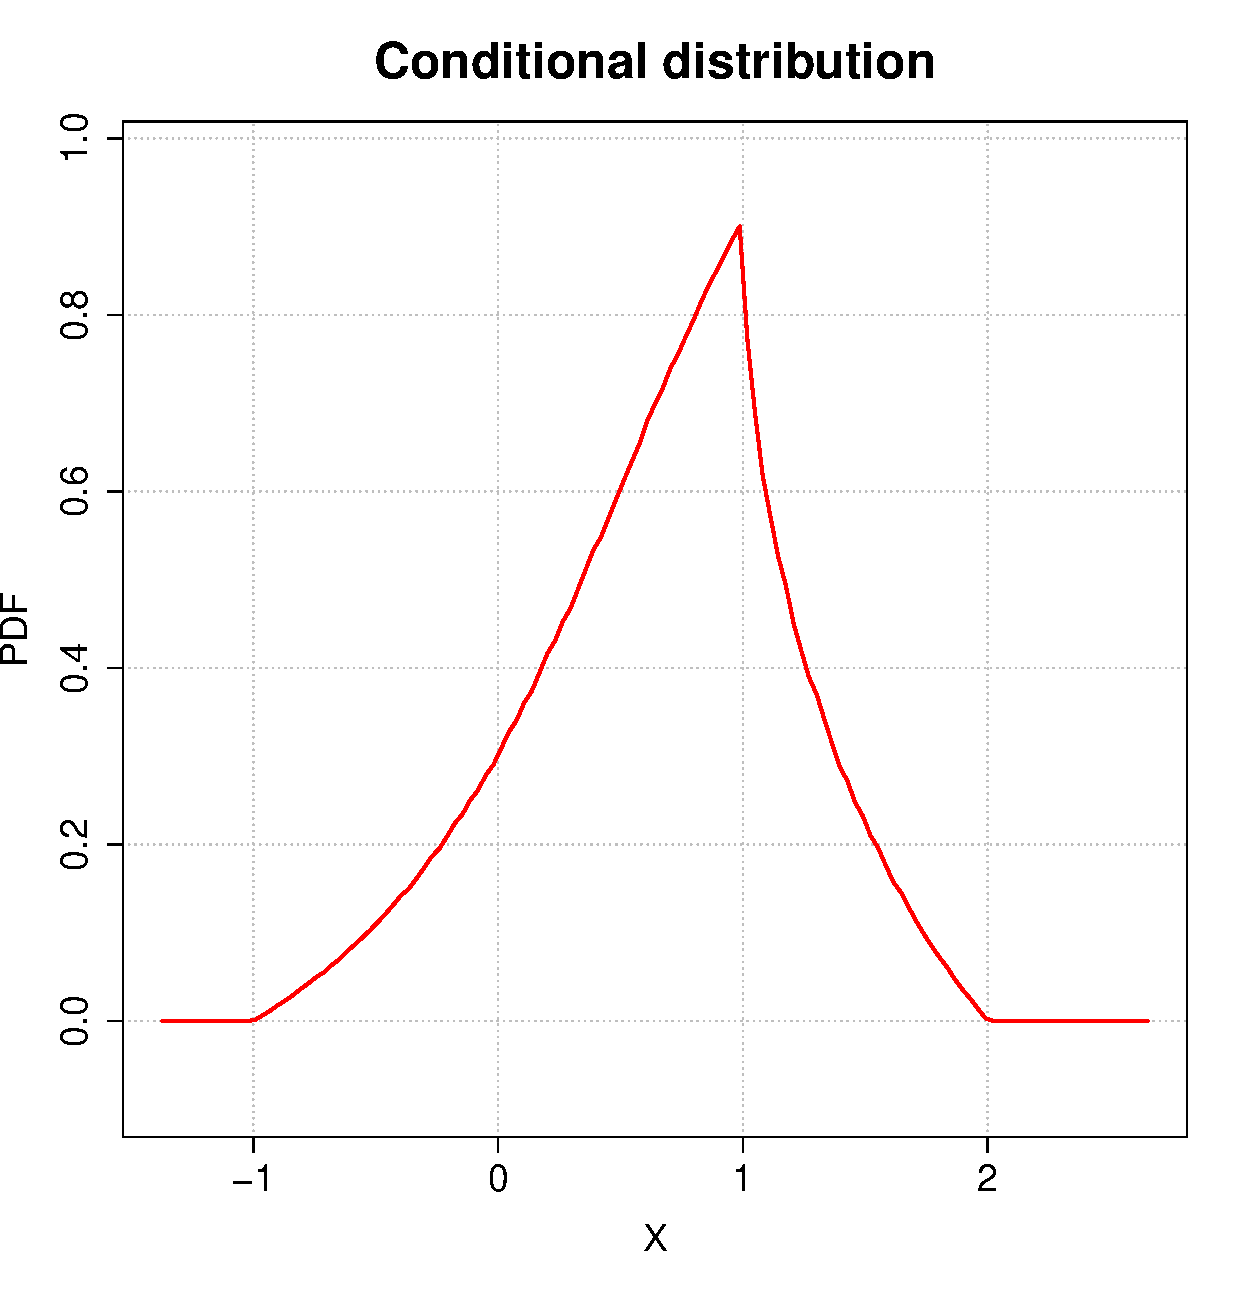
\includegraphics[width=7cm]{Figures/pdf_conditionalDist.pdf}
    \caption{$Uniform(Y, 1+Y^2)$ distribution with $Y\sim Uniform(-1,1)$.}
    \label{ConditionalPDF}
  \end{center}
\end{figure}
